\documentclass[palace_of_the_silver_princess]{subfiles}

\begin{document}
\fontfamily{ppl}\selectfont
\clearpage

\twocolumn[{\section{Part 4: Key To The Upper Level}}]
\markright{Part 4: Key To The Upper Level}

\subsubsection{1}
\begin{quotebox}
    This watch tower room has 6 windows overlooking the surrounding
    lands. A trap door is in the center of the floor. A rope ladder lies
    to one side of it. Several arrows are embedded into the door, and a
    broken bow and a sword lay beside it.  There is a door in the east
    wall.
\end{quotebox}

After a round the players will hear scuffling and fighting noises from
the other side of the east wall door. Phrases like “Come on Briardoor, I
got her,” “no Joshua, not him” and “take that you filthy worm,” will be
heard intermixed with the other noises. If the players open the door to
investigate, bright light will fill the hallway, and all that will be
seen are three swords fighting each other as if by themselves. It is an
illusion placed there by the palace magic user to frighten intruders who
may decide to enter through the tower. The illusion will not be dis-
pelled by touch. The trap doors leads down to room \textbf{EL 38}.

\subsubsection{2}
\begin{quotebox}
    This partly intact ancient laboratory holds the remains of several
    experiments, small scraps of paper, beakers, and a variety of other
    equipment spilled across onto two large oaken tables. A beautiful
    life-size green crystal statue of a gargoyle in the northeast
    corner. A polishing cloth is draped over its shield. An empty
    bookcase is leaning against the north wall, and a destroyed bookcase
    lies on the floor near the south wall.
\end{quotebox}

The crystal gargoyle is actually a living statue and was placed here long
ago. It still serves its purpose: to defend the lab from anyone who
enters. Three scraps of paper from the pile on the tables contain spells
for a 1st level magic user (spells to be determined by the DM).

\begin{monsterbox}{Gargoyle}
    \index[monsters]{Gargoyle}
	\textit{Medium elemental, chaotic evil}\\
	\hline
	\basics[
		armorclass = {15},
		hitpoints = {52 (7d8 + 21)},
		speed = {30~ft., fly 60~ft.}]
	\hline
	\stats[
		STR = \stat{15},
		DEX = \stat{11},
		CON = \stat{16},
		INT = \stat{6},
		WIS = \stat{11},
		CHA = \stat{7}]
	\hline
	\details[
        damageresistances = {bludgeoning, piercing, and slashing from nonmagicalweapons that aren't adamantine},
        damageimmunities = {poison},
        conditionimmunities = {exhaustion, petrified, poisoned},
		senses = {darkvision 60~ft., passive Perception 11},
		languages = {Terran},
		challenge = {2 (450 XP)}]
	\hline
	\begin{monsteraction}[False Appearance]
		While the gargoyle remains motionless, it is indistinguishable
        from an inanimate statue.
	\end{monsteraction}
	\monstersection{Actions}
	\begin{monsteraction}[Multiattack]
		The gargoyle makes two attacks: one with its bite
        and one with its claws.
	\end{monsteraction}

    \begin{monsteraction}[Bite]
		\textit{Melee Weapon Attack:} +4 to hit, reach 5ft., one target.

        \textit{Hit:} 5 (1d6 + 2) piercing damage.
	\end{monsteraction}

    \begin{monsteraction}[Claws]
		\textit{Melee Weapon Attack:} +4 to hit, reach 5 ft., one
        target.

        \textit{Hit:} 5 (1d6 + 2) slashing damage.
	\end{monsteraction}
\end{monsterbox}

\subsubsection{3}
\begin{quotebox}
    This is a deserted room. It is now empty.
\end{quotebox}

This room once held stores of various sorts but has long since been
cleaned out.

\textbf{Monster:}
\\
\\
\\
\textbf{Treasure:}
\\
\\
\\

\subsubsection{4}
\begin{quotebox}
    A plain, single bed and a huge wooden and metal desk dominate this
    sparsely furnished bedchamber. A broom lies in one corner near a
    pile of dirt.  A tattered pair of silk bedroom slippers lie at the
    floor of the plain bed. A small chest of drawers with attached
    mirror has been turned over.
\end{quotebox}

Hiding under the bed is a small black cat. It will appear as a harmless
domesticated creature, but is actually an enchanted great cat and can
become a panther once every other hour for 10 rounds. When in small cat
form it is harmless. It will be up to the DM to keep track of the
elapsed time and determine at what times the cat will transform itself.

Sewn into the mattress of the bed are \textbf{50 gold coins} and
\textbf{3 oval shaped rubies} worth 70 gp each.

\begin{monsterbox}{Cat}
    \index[monsters]{Cat}
	\textit{Tiny beast, unaligned}\\
	\hline
	\basics[
		armorclass = {12},
		hitpoints = {2 (1d4)},
		speed = {40~ft., climb 40~ft.}]
	\hline
	\stats[
		STR = \stat{3},
		DEX = \stat{15},
		CON = \stat{10},
		INT = \stat{3},
		WIS = \stat{12},
		CHA = \stat{7}]
	\hline
	\details[
        skills = {Perception +3, Stealth +4},
		senses = {passive Perception 13},
		languages = {---},
		challenge = {0 (10 XP)}]
	\hline
	\begin{monsteraction}[Keen Smell]
        The cat has advantage on Wisdom (Perception) checks that rely on
        smell.
	\end{monsteraction}
	\monstersection{Actions}
    \begin{monsteraction}[Claws]
		\textit{Melee Weapon Attack:} +0 to hit, reach 5 ft., one
        target.

        \textit{Hit:} 1 slashing damage.
	\end{monsteraction}
\end{monsterbox}

\begin{monsterbox}{Panther}
    \index[monsters]{Panther}
	\textit{Medium beast, unaligned}\\
	\hline
	\basics[
		armorclass = {12},
		hitpoints = {13 (3d8)},
		speed = {50~ft., climb 40~ft.}]
	\hline
	\stats[
		STR = \stat{14},
		DEX = \stat{15},
		CON = \stat{10},
		INT = \stat{3},
		WIS = \stat{14},
		CHA = \stat{7}]
	\hline
	\details[
        skills = {Perception +3, Stealth +6},
		senses = {passive Perception 14},
		languages = {---},
		challenge = {1/4 (50 XP)}]
	\hline
	\begin{monsteraction}[Keen Smell]
        The panther has advantage on Wisdom (Perception) checks that rely on
        smell.
	\end{monsteraction}

    \begin{monsteraction}[Pounce]
        If the panther moves at least 20 feet straight toward a creature
        and then hits it with a claw attack on the same turn, that
        target must succeed on a DC 12 Strength saving throw or be
        knocked prone. If the target is prone, the panther can make one
        bite attack against it as a bonus action.
	\end{monsteraction}
	\monstersection{Actions}
    \begin{monsteraction}[Bite]
		\textit{Melee Weapon Attack:} +4 to hit, reach 5 ft., one
        target.

        \textit{Hit:} 5 (1d6 + 2) piercing damage.
	\end{monsteraction}

    \begin{monsteraction}[Claw]
		\textit{Melee Weapon Attack:} +4 to hit, reach 5 ft ., one
        target.

        \textit{Hit:} 4 (1d4 + 2) slashing damage.
	\end{monsteraction}
\end{monsterbox}

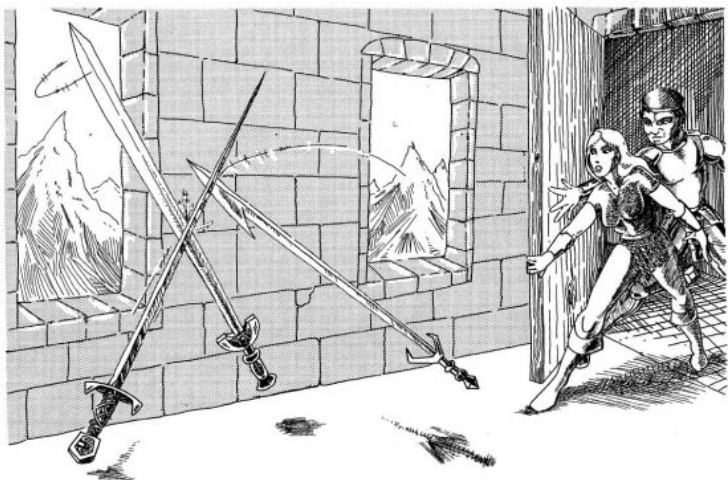
\includegraphics[width=\columnwidth]{img/trick_fight.png}

\subsubsection{5}
\begin{quotebox}
    This is a deserted room. It is empty.
\end{quotebox}

This room once held supplies and stores of various sorts but has long
since been emptied.

\textbf{Monster:}
\\
\\
\\
\textbf{Treasure:}
\\
\\
\\

\subsubsection{6}
\begin{quotebox}
    A huge, ornate, once lavishly decorated double canopy bed is
    directly across from the set of double doors. The bed posts
    resemble vines, nymphs, and birds all intertwined. The bed is
    covered in dusty, dull red velvet. Arrases line three of the walls
    with lovely and peaceful scenes of maidens riding on unicorns,
    playing in still pools that abound with plant life, and singing
    under starry skies lighted by a full moon. To either side of the
    door is a large hand carved chest of drawers, both with mirrors that
    are veined in silver. A small cushioned chair and matching footstool
    are at the end of the bed. On the footstool is a small makeup
    pallette and pestle.
\end{quotebox}

This was Lady Argenta’s room. It has remained untouched by man or
monster since the day she left it. The furniture and cloth here as well
as in the rest of the palace is rotten and of no value. All the drawers
have been emptied; and no clues or other information can be gained. The
makeup pallette is enameled in gold and was used for crushing colored
powders for eye makeup (1000 gp).

The view from the windows is into an overgrown garden.

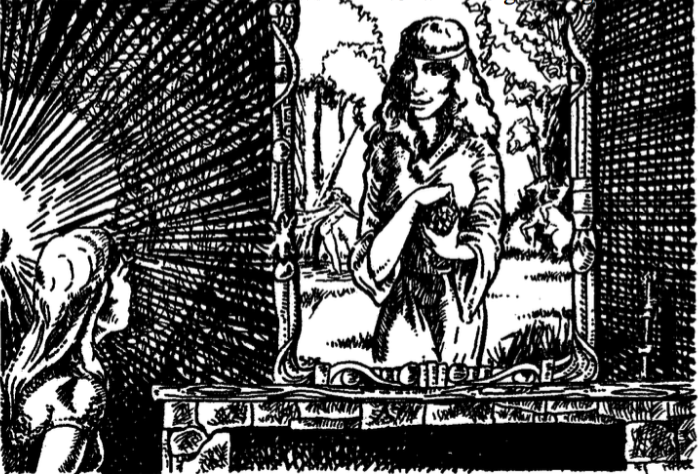
\includegraphics[width=\columnwidth]{img/lady.png}

\subsubsection{7}
\begin{quotebox}
    Several chairs and tables circle the fireplace in this room. A worn rug
    lies rolled up in one corner, and 3 knitting baskets sit beside it. On a
    small table near the fireplace is a small tea cup and saucer. Hanging
    over the fireplace is a portrait of Lady Argenta. She is holding a
    beautiful blood red ruby the size of an apple. Her smile betrays a hint
    of mischievousness.
\end{quotebox}

The only thing of value in the room is the tea cup. It is a magical
singing tea cup. When lifted off the saucer, the cup will begin to
randomly sing one of the 100 songs it knows.

\textbf{Monster:}
\\
\\
\\

\subsubsection{8}
\begin{quotebox}
    Shelves line this room. They are all empty now. A broken bedwarmer
    lays next to a small table and chair in the center of the room.
\end{quotebox}

\textbf{Monster:}
\\
\\
\\
\textbf{Treasure:}
\\
\\
\\
\textbf{Trap:}
\\
\\
\\

\subsubsection{9}
\begin{quotebox}
    This small room is lined with hangers and hooks. A chest of drawers
    is against the east wall.
\end{quotebox}

This was Lady Argenta’s closet. It is now empty of clothes or other
valuables.

\textbf{Monster:}
\\
\\
\\

\subsubsection{10}
\begin{quotebox}
    The walls of this lovely bathing room are painted with peaceful
    scenes of spring and summer. The ceiling and floor are mirrored and
    the floor retains some of its original polish. An ornate marble and
    silver enameled oval bathtub is against the eastern wall. A silver
    enameled towel rack standing next to the tub holds the remains of a
    thick towel and wash cloth. Many small and lovely soft soap
    containers are scattered randomly about the room. Bath oil pearls
    litter the now empty tub. At the head of the tub is a delicately
    sculpted tray centered with a small vase. It is decorated by three
    sets of three small gems. Each set of three is a different color —
    red, blue, and yellow.
\end{quotebox}

After one round, an ubue will enter from room \textbf{UL 11} to
investigate the noise in the bathing room. If there are more than 3
opponents, he will summon help from the remaining two ubues in room
\textbf{UL 11}. If the party is too strong, the monsters will retreat
into room \textbf{UL 11}.

The tray at the head of the tub is used to create water for bathing. The
magic works like this: Two red stones placed on the tray create hot
water, two yellow stones bring cold, and two blue ones remove it. Mix a
yellow and a red and the result is luke warm water. The blue ones only
work with each other. The tub will fill to capacity in 3 rounds. It will
empty in 1 round.

\begin{monsterbox}{Ubue}
    \index[monsters]{Ubue}
	\textit{Medium humanoid, true neutral}\\
	\hline
	\basics[
		armorclass = {10},
		hitpoints = {4 (1d8)},
		speed = {30~ft.}]
	\hline
	\stats[
		STR = \stat{10},
		DEX = \stat{10},
		CON = \stat{10},
		INT = \stat{10},
		WIS = \stat{10},
		CHA = \stat{10}]
	\hline
	\details[
		senses = {passive Perception 10},
		languages = {Common},
		challenge = {0 (10 XP)}]
	\hline
	\monstersection{Actions}
    \begin{monsteraction}[Club]
		\textit{Melee Weapon Attack:} +2 to hit, reach 5 ft., one
        target.

        \textit{Hit:} 2 (1d4) bludgeoning damage.
	\end{monsteraction}
\end{monsterbox}

\subsubsection{11}
\begin{quotebox}
    Three makeshift beds are lined against the south wall. A table with
    three chairs, and a huge stew pot sit near the fireplace. A tub
    filled with water and dishes is also near the fireplace. The walls
    are covered in portraits and other scenic paintings. Most of the
    portraits are of the Lady Argenta or of the Silver Warrior. One is
    of the red dragon, but it has been slashed in several places.
\end{quotebox}

This is the lair of three ubues. They have collected all the paintings
they could find to decorate the walls. The ubues are a family unit; one
of the ubues is female, and one is slightly smaller than the others.

The only thing of value in this room is the small chest of 40 gp hidden
under a loose brick in the fireplace.

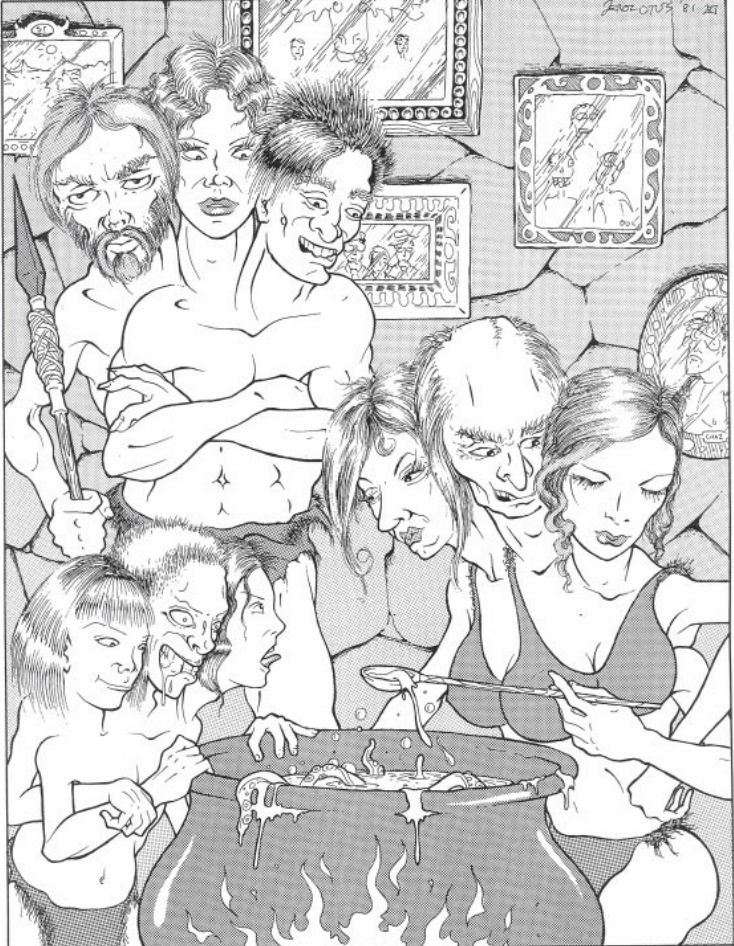
\includegraphics[width=\columnwidth]{img/ubues.png}

\subsubsection{12}
\begin{quotebox}
    This small room has only one stool and a table shoved out of the way
    against the north wall. There is a wheel on the south wall.
\end{quotebox}

This was a guard station. The wheel is used to lift the portcullis in
the hallway which is presently lowered. (A total of 20 strength points
will be needed to lift the portcullis if the wheel is not used.
Otherwise, one character with normal strength will be able to lift it.)

\textbf{Monster:}
\\
\\
\\
\textbf{Treasure:}
\\
\\
\\
\textbf{Trap:}
\\
\\
\\

\subsubsection{13}
\begin{quotebox}
    This garden is overgrown with weeds. The paths have disappeared into
    the underbrush, and the only statue is now completely grown over
    with thick purplish vines. Water can be heard, but not seen.
\end{quotebox}

Deadly plants for inhabit this plush garden, six \textbf{awakened
shrubs} near the statue and one \textbf{awakened tree}.  The shrubs will
attack anyone who comes near the statue, but the tree will only attack
if disturbed.

A fountain can be found by carefully searching near the southeast
corner of the garden. The fountain has healing powers that will cure
each person once and replace all lost hit points. Any attempts to use
the water again will not be successful, nor will the healing power of
the water remain if taken out of the fountain. The water must be drunk
or lapped up straight from the fountain.

\begin{figure*}[!ht]
    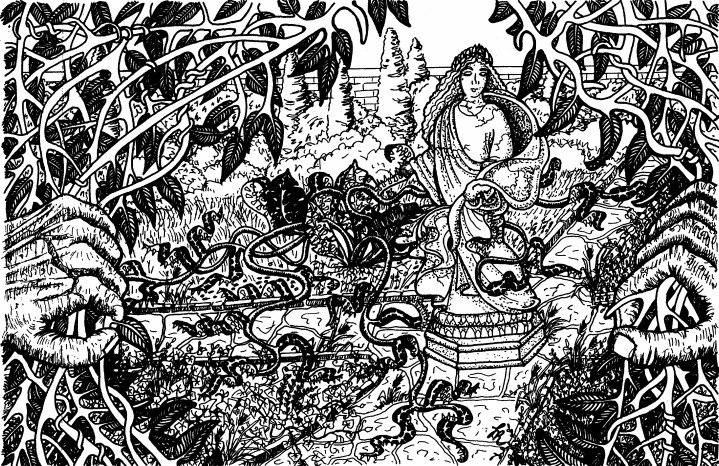
\includegraphics[width=\textwidth]{img/garden.png}
\end{figure*}

%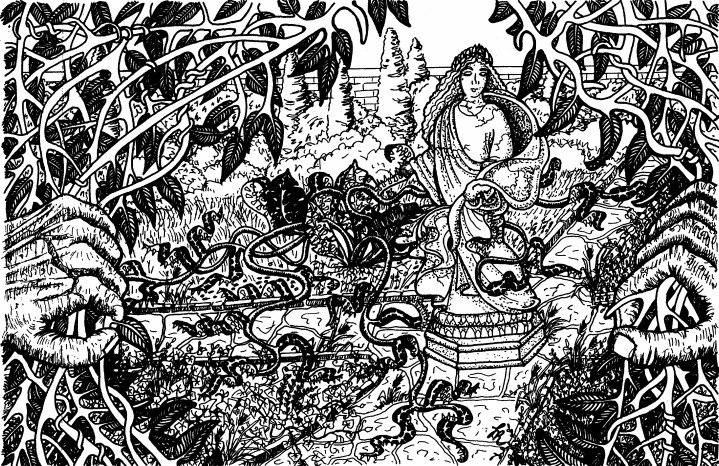
\includegraphics[width=\columnwidth]{img/garden.png}

\begin{monsterbox}{Awakened Shrub}
    \index[monsters]{Awakened Shrub}
	\textit{Small plant, unaligned}\\
	\hline
	\basics[
		armorclass = {9},
		hitpoints = {10 (3d6)},
		speed = {20~ft.}]
	\hline
	\stats[
		STR = \stat{3},
		DEX = \stat{8},
		CON = \stat{11},
		INT = \stat{10},
		WIS = \stat{10},
		CHA = \stat{6}]
	\hline
	\details[
        damagevulnerabilities = {fire},
        damageresistances = {piercing},
		senses = {passive Perception 10},
		languages = {Common},
		challenge = {0 (10 XP)}]
	\hline
	\begin{monsteraction}[False Appearance]
        While the shrub remains motionless, it is indistinguishable
        from a normal shrub.
	\end{monsteraction}

	\monstersection{Actions}
    \begin{monsteraction}[Rake]
		\textit{Melee Weapon Attack:} +1 to hit, reach 5ft., one target.

        \textit{Hit:} 1 (1d4 - 1) slashing damage.
	\end{monsteraction}
\end{monsterbox}

\begin{monsterbox}{Awakened Tree}
    \index[monsters]{Awakened Tree}
	\textit{Huge plant, unaligned}\\
	\hline
	\basics[
		armorclass = {13},
		hitpoints = {59 (7d12 + 14)},
		speed = {20~ft.}]
	\hline
	\stats[
		STR = \stat{19},
		DEX = \stat{6},
		CON = \stat{15},
		INT = \stat{10},
		WIS = \stat{10},
		CHA = \stat{7}]
	\hline
	\details[
        damagevulnerabilities = {fire},
        damageresistances = {bludgeoning, piercing},
		senses = {passive Perception 10},
		languages = {Common},
		challenge = {2 (450 XP)}]
	\hline
	\begin{monsteraction}[False Appearance]
        While the shrub remains motionless, it is indistinguishable
        from a normal shrub.
	\end{monsteraction}

	\monstersection{Actions}
    \begin{monsteraction}[Slam]
		\textit{Melee Weapon Attack:} +6 to hit, reach 10ft., one
        target.

        \textit{Hit:} 14 (3d6 + 4) bludgeoning damage.
	\end{monsteraction}
\end{monsterbox}

\subsubsection{14}
\begin{quotebox}
    Across from the double doors of this huge room stands a massive,
    hand carved wooden throne upon a dais. Two statues of warriors, one
    to either side of the throne, stand as silent guardians. In the
    center of the room are two huge columns. There are fire places on
    both the east and the west wall. Tapestries hang on the north wall.
    They record scenes of pomp and procession, royal galas and feasts
    once held in great halls. In the southeast and southwest corners are
    two more statues, duplicates of the ones guarding the throne.
\end{quotebox}

If the players linger here for more than one turn there is a 20\%
chance that 4-7 (1d4 + 3) ubues will enter through the double doors and
challenge the players’ right to be here. If no ubues are indicated,
check once for wandering monsters. If a wandering monster is
indicated, use the Wandering Monster Table in the front of the module.
If not, then no encounter will occur in this area.

\subsubsection{15}
\begin{quotebox}
    This room contains several couches. A small marble table and
    marble bench sit in front of the fire place. Thick layers of dust
    cover the furniture and floor.
\end{quotebox}

No one has been in this room since the palace was deserted by Lady
Argenta. DM Note: If the adventurers exploring this ruins have at least
two swords + 1 or a third level cleric, this room as well as room
\textbf{UL 16} would be an ideal location for the undead.

\subsubsection{16}
\begin{quotebox}
    This bedchamber has an eerie appearance. Dust and cobwebs cover
    everything so thickly that it is nearly impossible to distinguish
    exactly what furnishings are here.
\end{quotebox}

In this room is a bed, a large chest filled with old nightshirts, a
stool, and a wardrobe (empty). If the players venture into this room
their movement rate will be cut by \( \frac{1}{4} \) due to the thickness of the
dust and cobwebs. If the players spend more than 2 turns in this room an
image of an elf without feet or hands will appear floating above the bed
and remain there until someone sees him. When he is noticed, he will
smile cruelly and then move towards the person who first saw him, waving
his arms wildly. He will sweep down on the character, but not touch him
or her. This action will continue for three rounds after which time the
elf will disappear and all that will remain is laughter echoing off the
walls. When the laughter stops, the door will slam shut and lock. It
will take a combined strength total of 30 points to open the door once
it has been shut.

\subsubsection{17}
\begin{quotebox}
    A single pedestal with a glass case on top of it stands in the
    middle of this room. A small brown box with strange runes carved
    into it is inside the glass case.
\end{quotebox}

This is the room that holds the ruby known as "My Lady’s Heart." As soon
as the glass case is touched, both Lady Argenta and her knight in silver
and blue armor will appear. They are not illusions. They are ghasts 
and have come to protect the ruby. They will attack any person in the
room. 

\begin{monsterbox}{Lady Agenta / Knight In Silver (Ghasts)}
    \index[monsters]{Ghast}
    \index[monsters]{Lady Argenta}
    \index[monsters]{Knight in Silver and Blue}
	\textit{Medium undead, chaotic evil}\\
	\hline
	\basics[
		armorclass = {13},
		hitpoints = {36 (8d8)},
		speed = {30~ft.}]
	\hline
	\stats[
		STR = \stat{16},
		DEX = \stat{17},
		CON = \stat{10},
		INT = \stat{11},
		WIS = \stat{10},
		CHA = \stat{8}]
	\hline
	\details[
        damageresistances = {necrotic},
        damageimmunities = {poison},
        conditionimmunities = {charmed, exhaustion, poisoned},
		senses = {darkvision 60~ft.passive Perception 10},
		languages = {Common},
		challenge = {2 (450 XP)}]
	\hline
	\begin{monsteraction}[Stench]
        Any creature that starts its turn within 5 feet of the ghast
        must succeed on a DC 10 Constitution saving throw or be poisoned
        until the start of its next turn. On a successfu l saving throw,
        the creature is immune to the ghast's Stench for 24 hours.
	\end{monsteraction}

    \begin{monsteraction}[Turning Defiance]
        The ghast and any ghouls within 30 feet of it have advantage on
        saving throws against effects that turn undead.
    \end{monsteraction}

	\monstersection{Actions}
    \begin{monsteraction}[Bite]
		\textit{Melee Weapon Attack:} +3 to hit, reach 5 ft., one
        creature.

        \textit{Hit:} 12 (2d8 + 3) piercing damage.
	\end{monsteraction}

    \begin{monsteraction}[Claws]
		\textit{Melee Weapon Attack:} +5 to hit, reach 5 ft., one
        target.

        \textit{Hit:} 0 (2d6 + 3) slashing damage. If the target is a
        creature other than an undead, it must succeed on a DC 10
        Constitution saving throw or be paralyzed for 1 minute. The
        target can repeat the saving throw at the end of each of its
        turns, ending the effect on itself on a success.
	\end{monsteraction}
\end{monsterbox}

\subsubsection{18}
\begin{quotebox}
    A large pallet lies against the western wall near several large
    cushions. A chest and several smaller boxes line the north wall from
    comer to door. There is a fire burning in the fireplace and a large
    pot of horrible smelling food cooking in it.
\end{quotebox}

This room is filled with 7 male ubues.  The chief will ask why the party
is invading their lair. If the answer is unacceptable the ubues will
fight to protect their females and children (in room \textbf{19}). They
will retreat into room \textbf{19} if necessary. In this encounter only,
the players will not have time to examine the room before combat begins.
The room description should be read after the ubues have been defeated.

The only things of value in this area are \textbf{45 gp}, a
\textbf{silver bracelet} (3 gp), a \textbf{pearl necklace} (15 gp) and a
\textbf{music box} with a dancing couple on top (150 gp). These items
are inside a small chest at the north end of the room.

\begin{figure*}[!ht]
    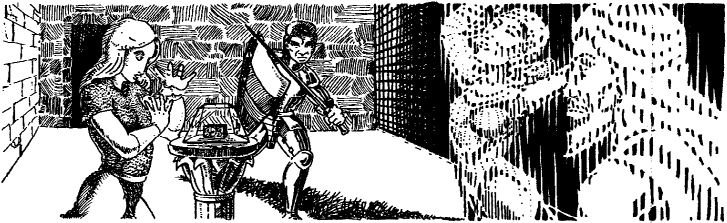
\includegraphics[width=\textwidth]{img/ruby_box.png}
\end{figure*}

\subsubsection{19}

Three female ubues and four ubue children are in this room.  The women
are working and the children are playing.  

If the players enter this area from the entrance level use this
description: One male ubue guard will be standing on the east side of
the door. If the intruders outnumber him 4 to 1, he will retreat and
sound the alarm. Room \textbf{UL 19} will be cleared of all females and
children and only the ubues from room \textbf{UL 18} will join the guard
and attack.

If the party enters from room \textbf{UL 18} the females will retreat
down the stairs, hoping to avoid a confrontation and to save the
children. They will fight if attacked. Once out the door, the females
will place a heavy iron bar against the door to keep the adventurers
from following.  Characters will have a 1 in 8 chance of preventing the
females from securing the door. It will take a combined strength of 25
to open the door once it has been secured. However, by the time the door
is opened, the females will already be down the stairs and gone. They
will bypass all rooms until they have reached the small worship area of
room \textbf{EL 15}.

If the characters enter from the hallway the adventurers will find the
females busily going about their tasks. Once the characters have
opened the door, and given the females a chance to see them, the ubues
will sound an alarm and then follow the actions outlined for escape.

A total of \textbf{13 cp}, 4 \textbf{silver bracelets} (2 gp each) a
\textbf{silver neck-chain} (1 sp) and three potions (healing) are in
various places in the room.

\subsubsection{20}
\begin{quotebox}
    This appears to be an empty room.
\end{quotebox}

\textbf{Monster:}
\\
\\
\\
\textbf{Treasure:}
\\
\\
\\
\textbf{Trap:}
\\
\\
\\
\subsubsection{21}
\textbf{Corridor:} As the party steps under this archway, they step on a
hidden pressure plate that rings an alarm bell in room \textbf{UL 22},
warning the monster there of the party’s presence.

\subsubsection{22}
\begin{quotebox}
    A beautiful young woman hangs from the ceiling. Nine
    ugly men can be seen poking their swords lightly into her flesh,
    all the while taunting her in an unknown language and pulling at
    what few clothes she has on. Part of her ankle length hair has
    been wrapped around her legs, securely binding them together,
    while the rest of her hair has been used to tie her hands to a
    ceiling beam. A long U shaped table dominates most of the floor
    space. A huge fireplace is on the north wall.
\end{quotebox}

There is no woman being tortured by nine men. It is an illusion produced
by the monster living in this room, a decapus.  It will attempt to lure
unsuspecting adventurers into its reach so that it may attack them. 

\textbf{One hundred silver pieces}, a \textbf{small pouch of rubies} (13
rubies, 10-40 (1d4x10) gp each) and a \textbf{silver tipped arrow} are
hidden under a loose stone in the fireplace.

\begin{monsterbox}{Decapus}
    \index[monsters]{Decapus}
	\textit{Huge monstrosity, chaotic evil}\\
	\hline
	\basics[
		armorclass = {12},
		hitpoints = {59 (7d12 + 15)},
		speed = {50~ft., climb 25~ft.}]
	\hline
	\stats[
		STR = \stat{10},
		DEX = \stat{15},
		CON = \stat{10},
		INT = \stat{7},
		WIS = \stat{10},
		CHA = \stat{9}]
	\hline
	\details[
		senses = {darkvision 60~ft.passive Perception 10},
		languages = {decapus},
		challenge = {2 (450 XP)}]
	\hline
	\begin{monsteraction}[Superior Hearing]
        The decapus makes all perception checks at advantage that deal
        with sound.
	\end{monsteraction}

    \begin{monsteraction}[Deceiving Illusion]
        The decapus can create a visual illusion up to 60~ft. away, with
        a radius of 20~ft.  This illusion is visual only, and does not
        have an auditory or olfactory aspect.
    \end{monsteraction}

    \begin{monsteraction}[Rend]
        If three tentacle attacks have hit a target in the same turn,
        the target is grappled until the start of the decapus' next
        turn, and will suffer 11 (2d8 + 2) damage from the creature's
        bite.  Only one opponent can be attacked per round this way.
    \end{monsteraction}

	\monstersection{Actions}
    \begin{monsteraction}[Multi-Attack]
        The decapus can make up to 9 tentacle attacks per round, up to 3
        on the same target.
	\end{monsteraction}

    \begin{monsteraction}[Tentacle]
		\textit{Melee Weapon Attack:} +4 to hit, range 10~ft., one
        creature.

        \textit{Hit:} 5 (1d6 + 1) bludgeoning damage.
	\end{monsteraction}
\end{monsterbox}

\subsubsection{23}
\begin{quotebox}
    This appears to be an empty room.
\end{quotebox}

It is recommended that no monster, treasure or trap be placed here.

\subsubsection{24}
\begin{quotebox}
    A statue of a young girl playing with a dove is in the southeastern
    corner of this oddly shaped room. A large handcarved bookcase stands
    next to the northeastern wall. Two wooden benches, one in front of
    each of the two windows facing southwest, have scrolls lying upon
    them. A dead potted tree sits in the northwest corner.
\end{quotebox}

Hidden in the tree pot are three strange looking eggs. They are shaped
much like oranges and have a bright red crystal shell.

Any character touching one of the eggs may sustain damage if the shell
is broken. The substance in the eggs can cause para- lyzation and a
character breaking the eggs will suffer 1-4 points of damage and must
make a save vs. Paralyzation at + 3. If removed from the nest, the eggs
will not hatch. It will be up to the DM to decide what laid the eggs.

The 13 scrolls are simply works of common reading. However, the bands
that hold them are pure silver (3 gp each).

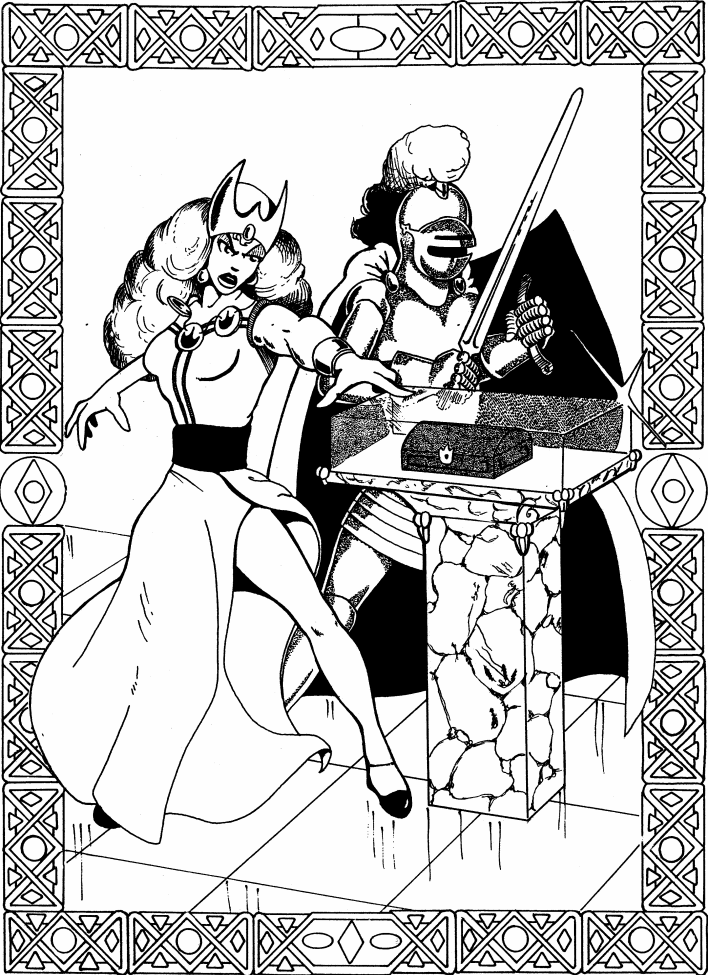
\includegraphics[width=\columnwidth]{img/ruby_box_2.png}

\begin{figure*}[!ht]
    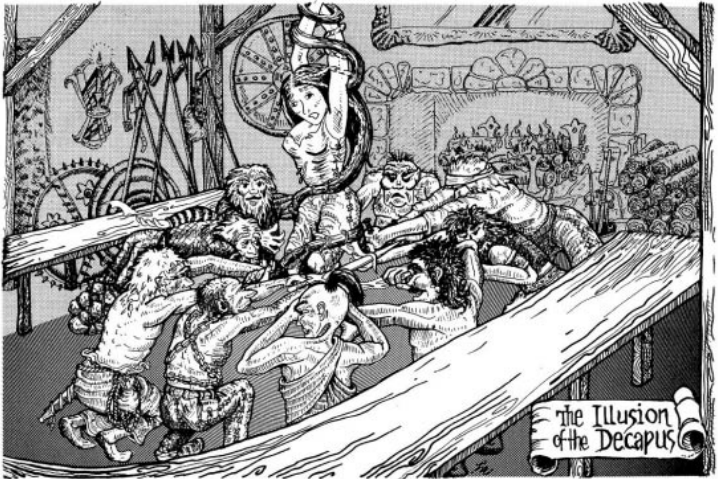
\includegraphics[width=\textwidth]{img/illusion.png}
\end{figure*}

\subsubsection{25}
\begin{quotebox}
    In this room is a massive canopy bed concealed behind thick dark red
    curtains, a long dresser with matching chest of drawers, and a
    large, stuffed easy chair. Three matching rugs lay side by side on
    the floor.
\end{quotebox}

This room is haunted by a poltergeist.  As soon as the characters have
entered, the curtains on the bed will begin to move as if someone were
occupying the bed. Though nothing will be discovered there, a man-like
form will appear to be in the bed under the covers. After 3 rounds have
passed, drawers will open and close, and the rugs will move about on
their own attempting to knock down adventurers who may be standing on
them. The easy chair will dance across the floor, then rise up into the
air and spin about for a round before crashing back down on the floor
where it originally stood. The decorative balls on the bedposts will
unscrew themselves and then float effortlessly in the air. They will
drop on an unarmored character’s head causing 1-4 points of damage per
hit. Finally dust will collect into a pile and then billow up into a
whirlwind causing characters to cough uncontrollably for 1-4 rounds
unless a DC 10 Constitution saving throw is made.

There is nothing of value in this room.

\begin{monsterbox}{Poltergeist}
    \index[monsters]{Poltergeist}
	\textit{Huge monstrosity, chaotic evil}\\
	\hline
	\basics[
		armorclass = {12},
		hitpoints = {22 (5d8)},
		speed = {0~ft., fly 50~ft.}]
	\hline
	\stats[
		STR = \stat{1},
		DEX = \stat{14},
		CON = \stat{11},
		INT = \stat{10},
		WIS = \stat{10},
		CHA = \stat{11}]
	\hline
	\details[
        damageresistances = {acid, cold, fire, lightning, thunder,
        bludgeoning, piercing, and slashing from nonmagical weapons},
        damageimmunities = {necrotic, poison},
        conditionimmunities = {charmed , exhaustion , grappled,
            paralyzed, petrified, poisoned, prone, restrained,
            unconscious},
		senses = {darkvision 60~ft.passive Perception 10},
		languages = {understands all the languages it knew in life but
        can't speak},
		challenge = {1 (200 XP)}]
	\hline
	\begin{monsteraction}[Invisibility]
        The poltergeist is invisible.
	\end{monsteraction}

	\monstersection{Actions}

    \begin{monsteraction}[Forceful Slam]
		\textit{Melee Weapon Attack:} +4 to hit, reach 5 ft.,
        one creature. 

        \textit{Hit:} 10 (3d6) force damage.
	\end{monsteraction}

    \begin{monsteraction}[Telekinetic Thrust]
        The poltergeist targets a creature or unattended object within
        30 feet of it. A creature must be Medium or smaller to be
        affected by this magic, and an object can weigh up to 150
        pounds.

        If the target is a creature, the poltergeist makes a Charisma
        check contested by the target's Strength check. If the
        poltergeist wins the contest, the poltergeist hurls the target
        up to 30 feet in any direction , including upward. Ifthe target
        then comes into contact with a hard surface or heavy object, the
        target takes 1d6 damage per 10 feet moved.

        If the target is an object that isn't being worn or carried, the
        poltergeist hurls it up to 30 feet in any direction.  The
        poltergeist can use the object as a ranged weapon, attacking one
        creature along the object's path (+4 to hit) and dealing 5 (2d4)
        bludgeoning damage on a hit.
    \end{monsteraction}
\end{monsterbox}

\begin{figure*}[!ht]
    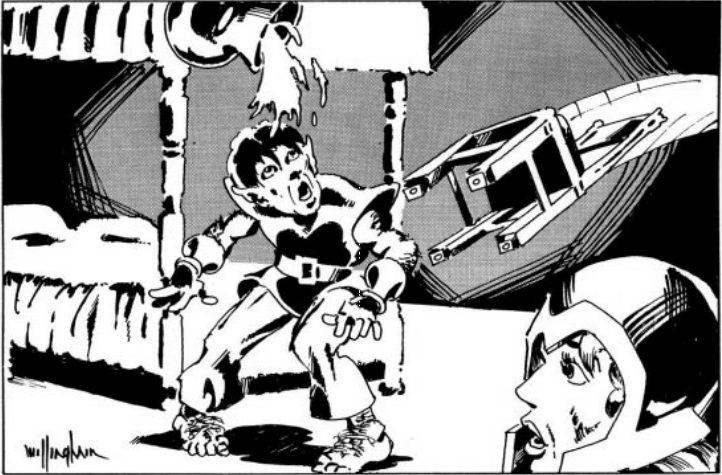
\includegraphics[width=\textwidth]{img/ghost.png}
\end{figure*}

\subsubsection{26}
\begin{quotebox}
    This small barred alcove looks into a temple room. There are two
    large cushioned chairs sitting here. A small book lies on the floor
    between them.
\end{quotebox}

The book was a prayer book, but is now just rotten leather and paper.

\textbf{Trap:}
\\
\\
\\

\subsubsection{27}
\begin{quotebox}
    This empty temple room is uneasily quiet. The dais on the west wall
    appears harmless, but seems to change, in some way, each time it is
    looked at. (The stairs seem to appear and disappear. The holy symbol
    seems to move about on the wall.) Faint whistling can be heard from
    time to time. It seems to almost have a melody.
\end{quotebox}

\textbf{Monster:}
\\
\\
\\
\textbf{Treasure:}
\\
\\
\\

\subsubsection{28}
\begin{quotebox}
    This room is filled with holy symbols from many different religions.
    A mace hangs on the walls between two windows that open onto the
    surrounding lands. The windows face northwest.
\end{quotebox}

After one round, a secret door will open on the east wall.
Catharandamus, a cleric will step out and challenge the players. He will
want to know why they are in his domain.

If Catharandamus is satisfied with the party’s answers, he will appear
to be friendly. He may ask for an offering. He may also sell the party
one bottle of \textbf{Anterian Brandy}, as this would appeal to his
sense of humor. He might even ask the party to join him!  (if the party
agrees, they become his retainers and the DM can develop the campaign
from there — the party may even end up defending the palace from NPC
parties!)

If he is not satisfied with their answers he’ll announce that he will
attack if they do not leave now. His spells are cause fear, darkness.
When he announces that he will attack, two dwarves and a female werebear
will step out from the secret door to join him. The dwarves, Xyzom
and Boron will move out first, letting Aleigha follow.  Her sword is the
Sword of Spartusia, a magic ruby bladed weapon that in her hands
functions as a sword + 2. In any one else's hands it will function only
as a sword + 1. 

The treasure owned by the four is in the secret room. It consists of
400 gp, 1000 sp, a pouch of fire agates (5 gp each), a potion of ESP,
and 15 bottles of Anterian Brandy (250 gp each).

\begin{monsterbox}{Catharandamus}
    \index[monsters]{Catharandamus}
    \textit{Medium humanoid (human), lawful evil}\\
	\hline
	\basics[
		armorclass = {13},
		hitpoints = {27 (5d8 + 5)},
		speed = {25~ft.}]
	\hline
	\stats[
		STR = \stat{10},
		DEX = \stat{10},
		CON = \stat{12},
		INT = \stat{13},
		WIS = \stat{16},
		CHA = \stat{13}]
	\hline
	\details[
        skills = {Medicine +7, Persuasion +3, Religion +4},
		senses = {passive Perception 13},
        languages = {Common, Dwarvish},
		challenge = {2 (450 XP)}]
	\hline
    \begin{monsteraction}[Cantrips]
        Fear, darkness
    \end{monsteraction}

	\monstersection{Actions}

    \begin{monsteraction}[Mace]
        \textit{Melee Weapon Attack:} +2 to hit, reach 5ft., one target. 

        \textit{Hit:} 3 (1d6) bludgeoning damage.
    \end{monsteraction}
\end{monsterbox}

\begin{monsterbox}{Xyzom \& Boron}
    \index[monsters]{Xyzom}
    \index[monsters]{Boron}
    \textit{Medium humanoid (dwarf), lawful neutral}\\
	\hline
	\basics[
		armorclass = {16},
		hitpoints = {26 (4d8 + 8)},
		speed = {25~ft.}]
	\hline
	\stats[
		STR = \stat{14},
		DEX = \stat{11},
		CON = \stat{14},
		INT = \stat{11},
		WIS = \stat{10},
		CHA = \stat{9}]
	\hline
	\details[
		senses = {passive Perception 10},
        languages = {Common, Dwarvish},
		challenge = {1 (200 XP)}]
	\hline
	\monstersection{Actions}

    \begin{monsteraction}[War Pick]
        \textit{Melee Weapon Attack:} +4 to hit, reach 5ft., one target. 

        \textit{Hit:} 6 (1d8 + 2) piercing damage
    \end{monsteraction}
\end{monsterbox}

\begin{monsterbox}{Aleigha}
    \index[monsters]{Aleigha}
    \textit{Medium humanoid (human, shapechanger), neutral good}\\
	\hline
	\basics[
        armorclass = {10 in humanoid form, 11 (natural armor) in bear
        and hybrid form},
        hitpoints = {135 (18d8 +54)},
        speed = {30~ft. (40!ft., climb 30~ft. in bear or hybrid form)}]
	\hline
	\stats[
		STR = \stat{19},
		DEX = \stat{10},
		CON = \stat{17},
		INT = \stat{11},
		WIS = \stat{12},
		CHA = \stat{12}]
	\hline
	\details[
        skills = {Perception +7},
        damageimmunities = {bludgeoning, piercing, and slashing
        damage from nonmagical weapons th at aren't silvered},
		senses = {passive Perception 17},
        languages = {Common (can't speak in bear form)},
		challenge = {5 (1,800 XP)}]
	\hline
    \begin{monsteraction}[Shapechanger]
        The werebear can use its action to polymorph into a Large
        bear-humanoid hybrid or into a Large bear, or back into its true
        form, which is humanoid. Its statistics, other than its size amd
        AC, are the same in each form. Any equipment it is wearing or
        carrying isn't transformed· It reverts to its true form if it dies.
    \end{monsteraction}

	\monstersection{Actions}

    \begin{monsteraction}[Multiattack]
        In bear form, the werebear makes two claw
        attacks. In humanoid form, it makes two greataxe attacks. In
        hybrid form, it can attack like a bear or a humanoid.
    \end{monsteraction}

    \begin{monsteraction}[Bite (Bear or Hybrid Form Only)]
        \textit{Melee Weapon Attack:} +7 to hit, reach 5 ft., one target.

        \textit{Hit:} 15 (2d10 + 4) piercing damage.  If the target is a
        humanoid, it must succeed on a DC 14 Constitution saving throw
        or be cursed with were bear lycanthropy.
    \end{monsteraction}

    \begin{monsteraction}[Claw (Bear or Hybrid Form Only)]
        \textit{Melee Weapon Attack:} +7 to hit, reach 5 ft., one target.

        \textit{Hit:} 13 (2d8 + 4) slashing damage.
    \end{monsteraction}

    \begin{monsteraction}[Sword of Spartusia]
        \textit{Melee Weapon Attack:} +7 to hit, reach 5 ft., one target.

        \textit{Hit:} 10 (1d12 + 4) slashing damage.
    \end{monsteraction}
\end{monsterbox}


\subtitlesection{Sword of Spartusia}
{Weapon, rare}
\index[magic]{Sword of Spartusia}

This wondrous, ruby-bladed magic sword once belonged to the legendary
female warrior Spartusia Ericsdottir. The sword is believed to be
cursed; a curse that caused it to constantly search for a true female
descent of Spartusia. The sword has had many owners, most of whom died
horrible or embarrassing deaths. Recently there have been stories of
the sword reemerging from unknown depths, and it is now in the hands of
a female werebear. It functions as a + 2 weapon in the hands of
Spartusia’s descendant, all others find that it will serve only at + 1.
Males find the sword’s build a little too delicate and feminine, but it
seems perfect for the hand of a strong female.

\begin{figure*}[!ht]
    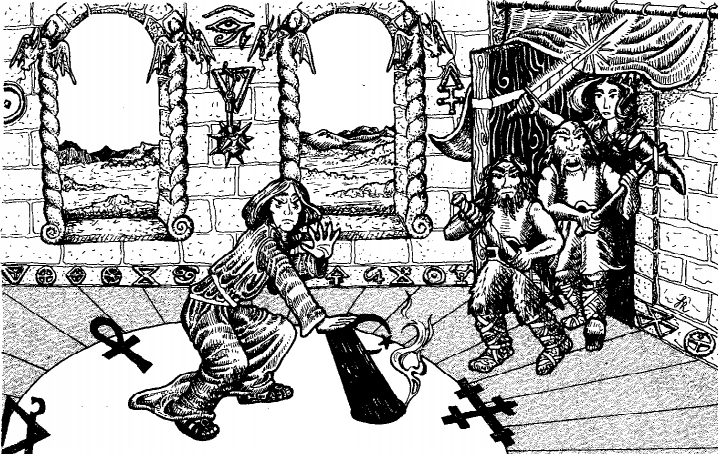
\includegraphics[width=\textwidth]{img/cleric.png}
\end{figure*}

\subtitlesection{Anterian Brandy}
{Item, rare}
\index[magic]{Anterian Brandy}

A heavenly drink made by dwarves skilled in the art of brewing. The
secret of how Anterian Brandy is made is guarded as though it were worth
a fortune in gold. Since it is made by dwarves, it is natural for all
dwarves to love this cobalt blue, naturally cool, sweet-smelling liquor.
Once tasted, the drinker finds that he or she has become addicted to it,
won’t sell it and does his or her best to find some more. Only elves are
not affected by its habit-forming flavor, but will drink it anyway to
enjoy the delicious taste. Many an elf has drunk a stout,
hearty-drinking dwarf under the table.

The first ounce will cause the drinker to fall into a drunken stupor.
After recovering from the first drink, the consumer can slowly begin to
drink additional amounts of brandy before over-doing. After
successfully drinking a gallon of the brew, the drunken stupors will
cease, and the drinker will be able to enjoy this elixir as if it were a
normal brandy.

\subsubsection{29}
\begin{quotebox}
    This large ball room appears to have at one time been decorated in
    silver, red and blue. Two huge fireplaces, one on the west and the
    other on the east wall, hold the petrified remains of beasts that
    were once cooked in them; a couple of pigs, a deer and a side of
    beef. A huge ornate brass bell hangs down from the ceiling and is
    supported by 4 columns of white marble. Whistling sounds can be
    heard. They have a very pleasant melody.
\end{quotebox}

The whistle is coming from a giant marble snake hiding in the wire bell.
Its whistle has an effect much like a charm spell, and everyone who
hears it must make a save or be charmed by the snake.

\begin{monsterbox}{Giant Marble Snake}
    \index[monsters]{Giant Marble Snake}
	\textit{Huge beast, unaligned}\\
	\hline
	\basics[
		armorclass = {12},
		hitpoints = {60 (8d12 + 8)},
		speed = {30~ft., swim 30~ft.}]
	\hline
	\stats[
		STR = \stat{19},
		DEX = \stat{14},
		CON = \stat{12},
		INT = \stat{1},
		WIS = \stat{10},
		CHA = \stat{3}]
	\hline
	\details[
        skills = {Perception +2},
		senses = {blindsight 10~ft.passive Perception 12},
        languages = {---},
		challenge = {2 (450 XP)}]
	\hline
	\monstersection{Actions}

    \begin{monsteraction}[Bite]
		\textit{Melee Weapon Attack:} +6 to hit, reach 10ft., one
        creature.

        \textit{Hit:} 11 (2d6 +4) piercing damage.
	\end{monsteraction}

    \begin{monsteraction}[Constrict]
        \textit{Melee Weapon Attack:} +6 to hit, reach 5 ft., one
        creature. 

        \textit{Hit:} 13 (2d8 + 4) bludgeoning damage, and the target is
        grappled (escape DC 16). Until this grapple ends, the creature
        is restrained, and the snake can't constrict another target.
    \end{monsteraction}
\end{monsterbox}

\subsubsection{30}
\begin{quotebox}
    This balcony is blocked by vines and thorn bushes.
\end{quotebox}

If the players decide to enter the balcony, they will be attacked by an
awakened shrub lurking there.

\subsubsection{31}
\begin{quotebox}
    This small, quaint little room has a game table in the center. A
    chess set, with a game apparently in progress (or never finished),
    sits upon it. A large map of a world unknown to the adventurers has
    been painted on the floor. Little metal figures are placed on
    several of the countries. There is a win- dow on the west wall. A
    fireplace on the south wall has fresh logs in it.
\end{quotebox}

This room is a game and recreation room for Catharandamus and his
friends. The chess pieces are gold and silver plated (2000 gp). There is
a bottle of Anterian Brandy (250 gp) sitting on the mantle of the
fireplace. Catharandamus and his friends inhabited this room also. They
were all fond of playing games. A meerschaum carved bowl pipe (30 gp)
and an empty goblet lie on one side of the table, an empty wine glass
and a peacock fan lie on the other side of the table.

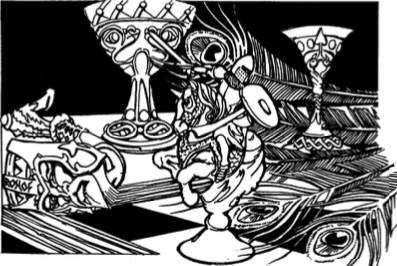
\includegraphics[width=\columnwidth]{img/goblet.png}




\end{document}
